\documentclass[ignorenonframetext,]{beamer}
\setbeamertemplate{caption}[numbered]
\setbeamertemplate{caption label separator}{: }
\setbeamercolor{caption name}{fg=normal text.fg}
\beamertemplatenavigationsymbolsempty
\usepackage{lmodern}
\usepackage{amssymb,amsmath}
\usepackage{ifxetex,ifluatex}
\usepackage{fixltx2e} % provides \textsubscript
\ifnum 0\ifxetex 1\fi\ifluatex 1\fi=0 % if pdftex
  \usepackage[T1]{fontenc}
  \usepackage[utf8]{inputenc}
\else % if luatex or xelatex
  \ifxetex
    \usepackage{mathspec}
  \else
    \usepackage{fontspec}
  \fi
  \defaultfontfeatures{Ligatures=TeX,Scale=MatchLowercase}
\fi
\usetheme[]{Singapore}
\usefonttheme{serif}
% use upquote if available, for straight quotes in verbatim environments
\IfFileExists{upquote.sty}{\usepackage{upquote}}{}
% use microtype if available
\IfFileExists{microtype.sty}{%
\usepackage{microtype}
\UseMicrotypeSet[protrusion]{basicmath} % disable protrusion for tt fonts
}{}
\newif\ifbibliography
\hypersetup{
            pdftitle={Module 2, Part 1: Statistical Learning},
            pdfauthor={Stefanie Muff, Department of Mathematical Sciences, NTNU},
            colorlinks=true,
            linkcolor=Maroon,
            citecolor=Blue,
            urlcolor=blue,
            breaklinks=true}
\urlstyle{same}  % don't use monospace font for urls
\usepackage{longtable,booktabs}
\usepackage{caption}
% These lines are needed to make table captions work with longtable:
\makeatletter
\def\fnum@table{\tablename~\thetable}
\makeatother
\usepackage{graphicx,grffile}
\makeatletter
\def\maxwidth{\ifdim\Gin@nat@width>\linewidth\linewidth\else\Gin@nat@width\fi}
\def\maxheight{\ifdim\Gin@nat@height>\textheight0.8\textheight\else\Gin@nat@height\fi}
\makeatother
% Scale images if necessary, so that they will not overflow the page
% margins by default, and it is still possible to overwrite the defaults
% using explicit options in \includegraphics[width, height, ...]{}
\setkeys{Gin}{width=\maxwidth,height=\maxheight,keepaspectratio}

% Prevent slide breaks in the middle of a paragraph:
\widowpenalties 1 10000
\raggedbottom

\AtBeginPart{
  \let\insertpartnumber\relax
  \let\partname\relax
  \frame{\partpage}
}
\AtBeginSection{
  \ifbibliography
  \else
    \let\insertsectionnumber\relax
    \let\sectionname\relax
    \frame{\sectionpage}
  \fi
}
\AtBeginSubsection{
  \let\insertsubsectionnumber\relax
  \let\subsectionname\relax
  \frame{\subsectionpage}
}

\setlength{\parindent}{0pt}
\setlength{\parskip}{6pt plus 2pt minus 1pt}
\setlength{\emergencystretch}{3em}  % prevent overfull lines
\providecommand{\tightlist}{%
  \setlength{\itemsep}{0pt}\setlength{\parskip}{0pt}}
\setcounter{secnumdepth}{0}
\usepackage{xcolor}

\title{Module 2, Part 1: Statistical Learning}
\subtitle{TMA4268 Statistical Learning V2020}
\author{Stefanie Muff, Department of Mathematical Sciences, NTNU}
\date{January 10, 2020}

\begin{document}
\frame{\titlepage}

\begin{frame}

Last update: January 07, 2020

\end{frame}

\begin{frame}{Acknowledgements}

\begin{itemize}
\item
  A lot of this material stems from Mette Langaas and her TAs (especiall
  Julia Debik). I would like to thank Mette for the permission to use
  her material!
\item
  Some of the figures and slides in this presentation are taken (or are
  inspired) from James et al. (2013).
\end{itemize}

\end{frame}

\begin{frame}{Introduction}

\begin{block}{Learning material for this module}

\begin{itemize}
\tightlist
\item
  James et al (2013): An Introduction to Statistical Learning. Chapter 2
  (except 2.2.3).\\
\item
  Additional material (in this module page) on random variables,
  covariance matrix and the multivariate normal distribution (known for
  students who have taken TMA4267 Linear statistical models).
\end{itemize}

\end{block}

\end{frame}

\begin{frame}

\begin{block}{What will you learn?}

\vspace{2mm}

\begin{itemize}
\item
  Statistical learning and examples thereof \vspace{1mm}
\item
  Introduce relevant notation and terminology \vspace{1mm}
\item
  Prediction accuracy vs.~model interpretability \vspace{1mm}
\item
  Bias-variance trade-off \vspace{1mm}
\item
  The basics of random vectors, covariance matrix and the multivariate
  normal distribution.
\end{itemize}

\end{block}

\end{frame}

\begin{frame}{What is statistical learning?}

\emph{Statistical learning} is the process of learning from data.

By applying \emph{statistical methods} on a \emph{data set} (called the
\emph{training set}), we would like to

\begin{itemize}
\tightlist
\item
  \emph{draw conclusions} about the relations between the variables
  (\emph{\textcolor{red}{inference}}) or
\item
  \emph{find a predictive function} for new observations
  (\emph{\textcolor{red}{predition}}).
\end{itemize}

Also, we would like to find structures in the data that help us to learn
something about the real world.

Statistical learning plays a key role in many areas of science, finance
and industry.

\end{frame}

\begin{frame}{Key concepts (stats) and notation}

Todo (see M1L1notes.pdf)

\end{frame}

\begin{frame}

\begin{block}{Two variable types}

\vspace{2mm}

\textbf{Quantitative} variables are variables from a continuous set,
they have a numerical value.

\begin{itemize}
\tightlist
\item
  Examples: a person's weight, a company's income, the age of a
  building, the temperature outside, the level of precipitation etc.
\end{itemize}

\vspace{2mm}

\textbf{Qualitative} variables are variables from a discrete set, from a
set of \(K\) different classes/labels/categories.

\begin{itemize}
\item
  Examples: type of fruit \{apples, oranges, bananas, \ldots{}\}, sex
  \{male, female, other \}, education level.
\item
  Qualitative variables which have only two classes are called
  \emph{binary} variables and are usually coded by 0 (no) and 1 (yes).
\end{itemize}

\end{block}

\end{frame}

\begin{frame}{Examples of learning problems}

\begin{itemize}
\item
  To predict the price of a stock 3 months from now, based on company
  performance measures and economic data. Here the response variable is
  quantitative (price).
\item
  Spam detection for emails.
\item
  To identify the risk factors for Prostate cancer.
\item
  Estimating the risk that someone will suffer from a heart disease or
  heart attack, given knowledge about condition, behaviour, age, or
  demographic, diet and clinical measurements. Here the \emph{outcome is
  binary} (yes, no) with both qualitative and quantitative input
  variables.
\item
  Predict soemeone's body fat, given BMI, weight, age, etc.
\item
  Digit recognition.
\item
  Image recognition.
\end{itemize}

\end{frame}

\begin{frame}

\begin{block}{Example 1: Handwritten digit recognition}

\begin{itemize}
\tightlist
\item
  Aim: To identify the numbers in a handwritten ZIP code, from a
  digitized image.
\item
  Classification problem, where the response variable is categorical
  with classes \{0, 1, 2, \ldots{}, 9\}. \vspace{1mm}
\end{itemize}

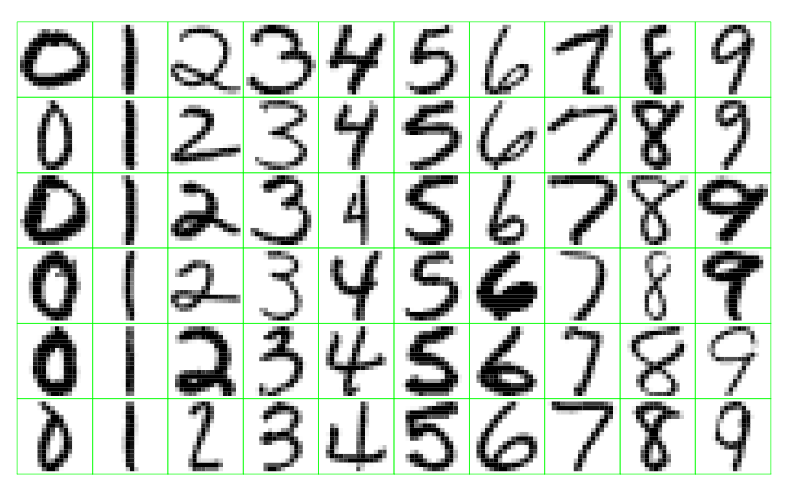
\includegraphics[width=0.70000\textwidth]{digits.png} \vspace{1mm}

Examples of handwritten digits from U.S. postal envelopes. \scriptsize
Image taken from \url{https://web.stanford.edu/~hastie/ElemStatLearnII/}

\end{block}

\end{frame}

\begin{frame}

\begin{block}{Example 2: Email classification (spam detection)}

\begin{itemize}
\tightlist
\item
  Goal: to build a spam filter.
\item
  This filter can based on the frequencies of words and characters in
  emails.
\end{itemize}

The table below show the average percentage of words or characters in an
email message, based on 4601 emails of which 1813 were classified as a
spam.

\begin{longtable}[]{@{}lrrrrrr@{}}
\toprule
& you & free & george & ! & \$ & edu\tabularnewline
\midrule
\endhead
not spam & 1.27 & 0.07 & 1.27 & 0.11 & 0.01 & 0.29\tabularnewline
spam & 2.26 & 0.52 & 0.00 & 0.51 & 0.17 & 0.01\tabularnewline
\bottomrule
\end{longtable}

\end{block}

\end{frame}

\begin{frame}

\begin{block}{Example 3: What makes a Nobel Prize winner?}

Perseverance, luck, skilled mentors or simply chocolate consumption? An
article published in the New England Journal of Medicine have concluded
with the following:

\begin{quote}
Chocolate consumption enhances cognitive function, which is a sine qua
non for winning the Nobel Prize, and it closely correlates with the
number of Nobel laureates in each country. It remains to be determined
whether the consumption of chocolate is the underlying mechanism for the
observed association with improved cognitive function.
\end{quote}

The figure shows the number of Nobel Laureates per 10 million population
against countries' annual per capita chocolate consumption.

You can read the article
\href{http://www.nejm.org/doi/full/10.1056/NEJMon1211064}{here} and a
informal review of the article
\href{https://blogs.scientificamerican.com/the-curious-wavefunction/chocolate-consumption-and-nobel-prizes-a-bizarre-juxtaposition-if-there-ever-was-one/}{here}.

\end{block}

\end{frame}

\begin{frame}

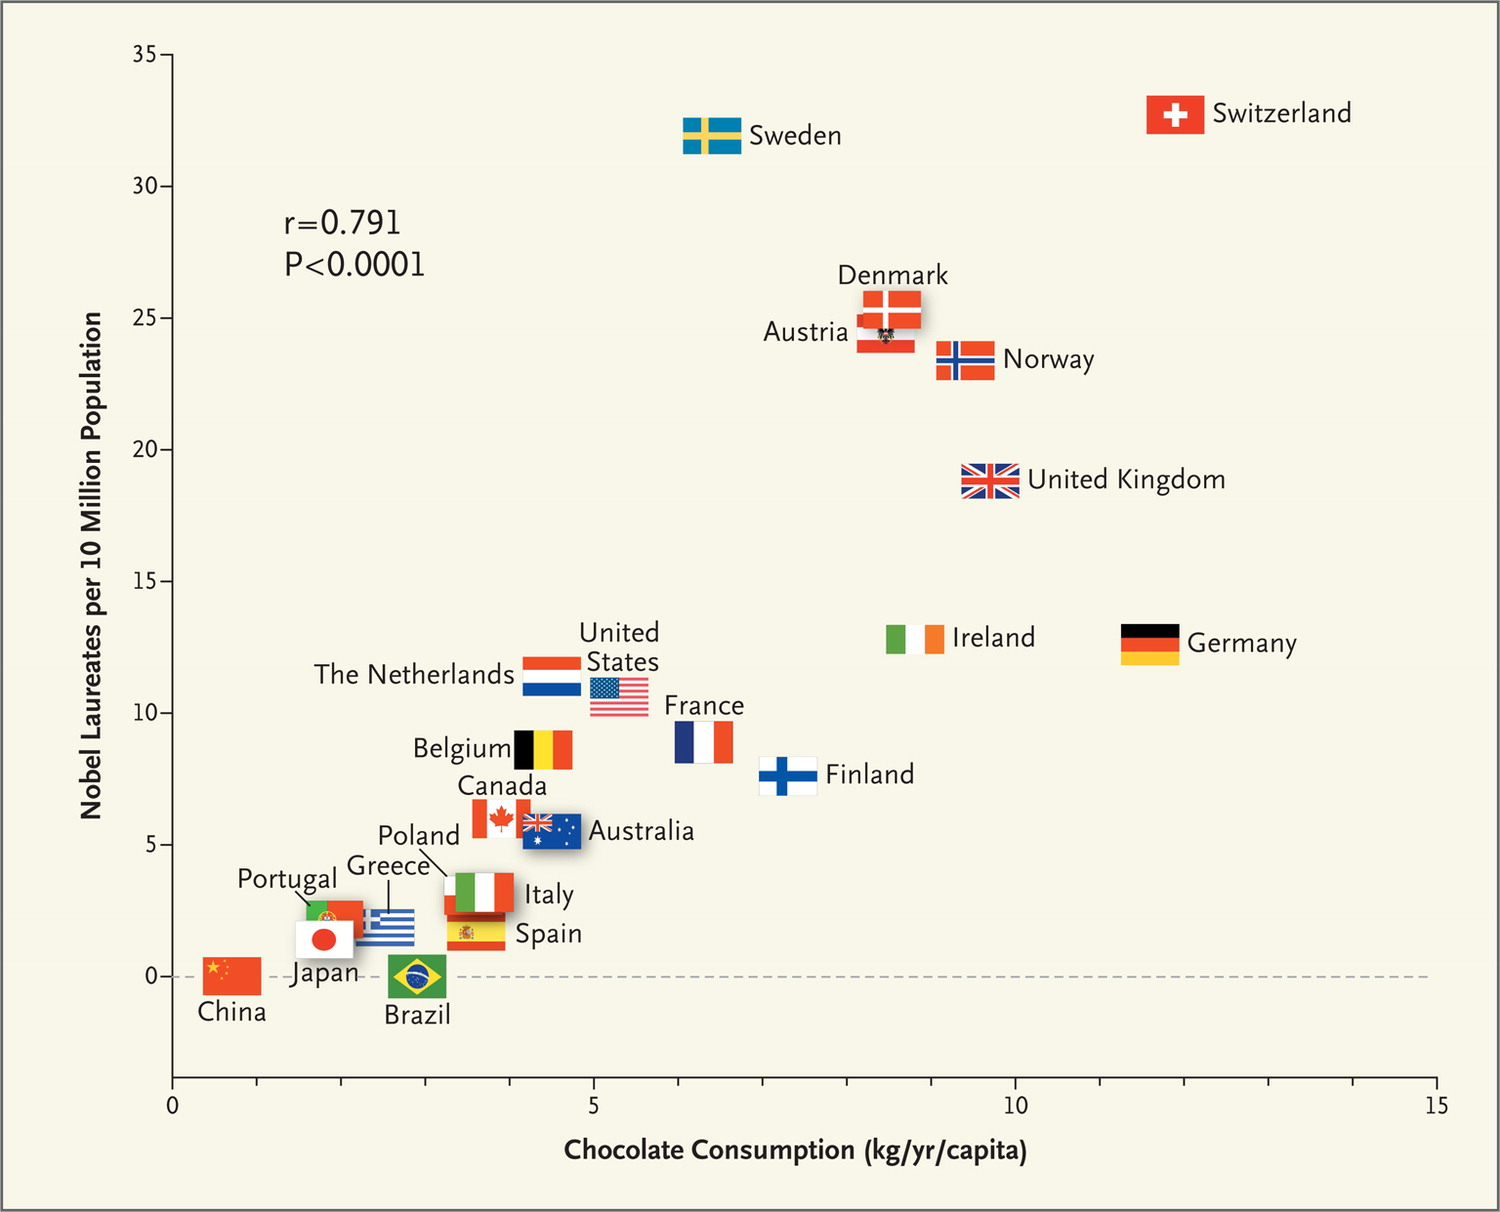
\includegraphics{chocolate.jpeg}

\end{frame}

\begin{frame}{The Supervised Learning Problem}

\textcolor{blue}{\emph{Starting point}}:

\begin{itemize}
\item
  Outcome measurement \(Y\), also called dependent variable, response,
  target.
\item
  Vector of \(p\) predictor measurements \(X=(X_1,\ldots,X_p)\), also
  called inputs, regressors, covariates, features, independent
  variables.
\item
  In the \textbf{regression problem}, \(Y\) is quantitative (e.g price,
  blood pressure).
\item
  In the \textbf{classification problem}, \(Y\) takes values in a
  finite, unordered set (survived/died, digit 0-9, cancer class of
  tissue sample).
\item
  We have training data \((x_1, y_1), \ldots , (x_N , y_N )\). These are
  observations (examples, instances) of these measurements.
\end{itemize}

\end{frame}

\begin{frame}

\begin{block}{Supervised learning and its objectives}

\vspace{2mm}

Our data set (training set) consists of \(n\) measurement of the
response variable \(Y\) and of \(p\) covariates \(x\):
\[(y_1, x_{11}, x_{12},\ldots, x_{1p}), (y_2, x_{21},\ldots, x_{2p}), \ldots, (y_n, x_{n1}, x_{n2},\ldots, x_{np}).\]
\(~\)

On the basis of the \emph{training data} we would like to:

\begin{itemize}
\item
  \textbf{accurately predict} unseen test cases.
\item
  \textbf{understand} which input affects the outcomes, and how.
\item
  \textbf{assess the quality} of your predictions and inference.
\end{itemize}

\vspace{2mm}

The majority of problems studied in this course fall in the supervised
learning category (exception: Module 10)

\end{block}

\end{frame}

\begin{frame}{The Unsupervised Learning Problem}

\begin{itemize}
\item
  There is \textbf{no outcome variable} \(y\), just a set of predictors
  (features) \(x_i\) measured on a set of samples.
\item
  Objective is more fuzzy -- find (hidden) patterns or groupings in the
  data - in order to \emph{gain insight and understanding}. There is no
  \emph{correct} answer.
\item
  Difficult to know how well your are doing.
\end{itemize}

Examples in the course:

\begin{itemize}
\tightlist
\item
  Clustering (M10)
\item
  Principal component analysis (M10)
\end{itemize}

\end{frame}

\begin{frame}{Overall philosophy}

\begin{itemize}
\item
  Important to understand the simpler methods first, in order to grasp
  the more sophisticated ones.
\item
  It is important to accurately assess the performance of a method, to
  know how well or how badly it is working.
\end{itemize}

\(\rightarrow\) \textbf{Simpler methods often perform as well as fancier
ones!}

\begin{itemize}
\item
  Statistical learning is a fundamental ingredient in the training of a
  modern data scientist.
\item
  It is an exciting research area, having important applications in
  science, industry and finance.
\end{itemize}

\end{frame}

\begin{frame}{Statistical Learning vs.~Machine Learning}

\begin{itemize}
\item
  Machine learning arose as a subfield of Artificial Intelligence.
\item
  Statistical learning arose as a subfield of Statistics.
\item
  There is much overlap --- both fields focus on supervised and
  unsupervised problems:

  \begin{itemize}
  \tightlist
  \item
    Machine learning has a greater emphasis on large scale applications
    and prediction accuracy.
  \item
    Statistical learning emphasizes models and their interpretability,
    and precision and uncertainty.
  \end{itemize}
\item
  The distinction has become more and more blurred, and there is a great
  deal of ``cross-fertilization''.
\item
  Machine learning has the upper hand in Marketing!
\end{itemize}

\end{frame}

\begin{frame}

\begin{itemize}
\item
  There is a controversy and some scepticism against ``too fancy'' ML
  methods.
\item
  Criticism: ML often re-invents existing methods and names them
  differently, but often without awareness of existing methods in
  statistics.
\item
  Almost weekly new literature that delivers comparison. Often, the
  ``simple'' statistical methods ``win''.
\end{itemize}

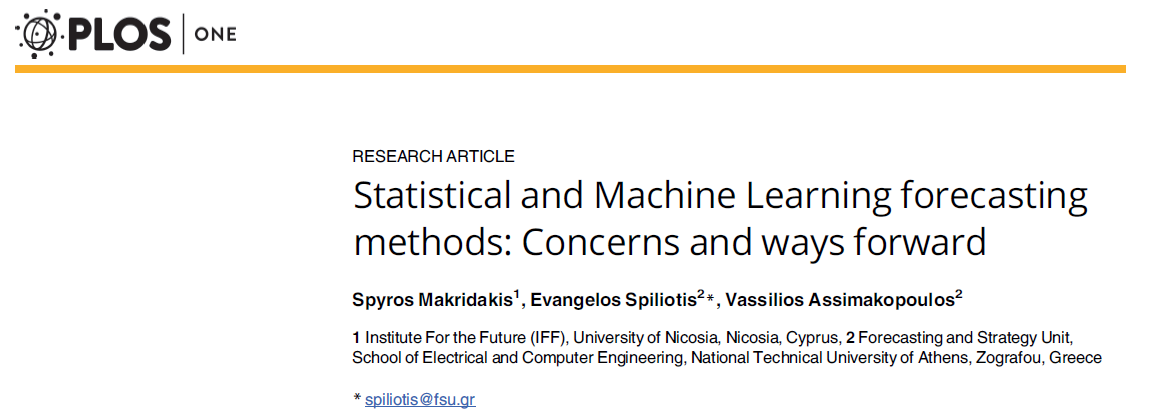
\includegraphics{ML_vs_stat.png}

\end{frame}

\begin{frame}

\begin{block}{What is the aim in statistical learning?}

\vspace{3mm}

Assume\footnote{We are talking about supervised methods now.}:

\begin{itemize}
\tightlist
\item
  we observe one \emph{quantitative} response \(Y\) and
\item
  \(p\) different predictors \(x_1, x_2,... , x_p\).
\end{itemize}

We assume that there is a function \(f\) that relates the response and
the predictor variables: \[ Y = f(x) + \varepsilon,\] where
\(\varepsilon\) is a random error term with mean 0 and independent of
\(x\).

\centering
{\bf The aim is to estimate $f$.}

\end{block}

\end{frame}

\begin{frame}{Example 1}

Sales of a product, given advertising budgets in different media.

\includegraphics{../../ISLR/Figures/Chapter2/2.1.png}

\end{frame}

\begin{frame}{Example 2}

\vspace{2mm} Income for given levels of education.

\includegraphics{../../ISLR/Figures/Chapter2/2.2.png}

\end{frame}

\begin{frame}

There are two main reasons for estimating \(f\):

\begin{itemize}
\item
  \textbf{Prediction}
\item
  \textbf{Inference}
\end{itemize}

\end{frame}

\begin{frame}

\begin{block}{Reason 1: Prediction}

\(~\)

\textbf{Aim}: predict a response \(Y\) given new observations \(x\) of
the covariates as accurately as possible.

\(~\) Notation:

\[\hat{Y} = \hat{f}(x).\]

\begin{itemize}
\item
  \(\hat{f}\): estimated \(f\)
\item
  \(\hat{Y}\) prediction for \(Y\) given \(x\).
\item
  We do not really care about the shape of \(f\) (``black box'').
  \(\rightarrow\) no interpretation of regression parameters when the
  aim is purely prediction!
\end{itemize}

\end{block}

\end{frame}

\begin{frame}

There are two quantities which influence the accuracy of \(\hat{Y}\) as
a prediction of \(Y\):

\begin{itemize}
\tightlist
\item
  The \emph{reducible error} has to do with our estimate \(\hat{f}\) of
  \(f\). This error can be reduced by using the most \emph{appropriate}
  statistical learning technique.
\item
  The \emph{irreducible error} comes from the error term \(\varepsilon\)
  and cannot be reduced by improving \(f\). This is related to the
  unobserved quantities influencing the response and possibly the
  randomness of the situation.
\end{itemize}

For a given \(\hat{f}\) and a set of predictors \(X\) which gives
\(\hat{Y}=\hat{f}(X)\), we have

\[\text{E}[(Y-\hat{Y})^2] = \underbrace{\text{E}[(f(X)-\hat{f}(X))^2]}_{reducible} + \underbrace{Var(\epsilon)}_{irreducible}\]

\end{frame}

\begin{frame}

\begin{block}{Q: If there were a \emph{deterministic} relationship
between the response and a set of predictors, would there then be both
reducible and irreducible error?}

\end{block}

\end{frame}

\begin{frame}

\begin{block}{Reason 2: Inference}

\(~\)

\textbf{Aim}: understand\_how the response variable is affected by the
various predictors (covariates).

\(~\)

The \emph{exact form} of \(\hat{f}\) is of \emph{main interest}.

\begin{itemize}
\tightlist
\item
  Which predictors are associated with the response?
\item
  What is the relationship between the response and each predictor?
\item
  Can the relationship be linear, or is a more complex model needed?
\end{itemize}

\end{block}

\end{frame}

\begin{frame}{Estimating \(f\)}

Overall idea:

\begin{itemize}
\tightlist
\item
  Using available \emph{training data} \((x_1,y_n),\ldots (x_n,y_n)\) to
  estimate \(\hat{f}\), such that \(Y\approx \hat{f}(X)\) for any
  \((X,Y)\) (also those that have not yet been observed).
\end{itemize}

Two main approaches:

\begin{itemize}
\tightlist
\item
  Parametric methods
\item
  Non-parametric methods
\end{itemize}

\end{frame}

\begin{frame}

\begin{block}{Parametric methods}

\(~\)

Asumption about the form or shape of the function \(f\).

The multiple linear model (M3) is an example of a parametric method:

\[f(x) = \beta_0 + \beta_1 x_1 + ... + \beta_p x_p+\varepsilon \ , \]

with \(\varepsilon \sim N(0,\sigma^2)\).

\(~\)

The task simplifies to finding estimates of the \(p+1\) coefficients
\(\beta_0, \beta_1, .. ,\beta_p\). To do this we use the training data
to fit the model, such that
\[Y \approx \hat{\beta_0} + \hat{\beta_1} x_1 + ... + \hat{\beta_p} x_p \ .\]

\end{block}

\end{frame}

\begin{frame}

Fitting a parametric models is thus done in two steps:

\begin{enumerate}
\def\labelenumi{\arabic{enumi}.}
\tightlist
\item
  Select a form for the function \(f\).\\
\item
  Estimate the unknown parameters in \(f\) using the training set.
\end{enumerate}

\end{frame}

\begin{frame}

\begin{block}{Non-parametric methods}

\(~\)

\begin{itemize}
\item
  Non-parametric methods seek an estimate of \(f\) that gets close to
  the data points, but without making explicit assumptions about the
  form of the function \(f\).
\item
  Example: \(K\)-nearest neighbour (KNN) algorithm, used in
  classification. KNN predicts a class membership for a new observation
  by making a majority vote based on its \(K\) nearest neighbours. We
  will discuss the \(K\)-nearest neighbour algorithm in Module 4.
\end{itemize}

(Todo: For the exercises make sure no KNN questions are in RecEx2 -- I
moved all this to module 4, because it was otherwise resdundant. You can
also move the respective questions to RecEx4, if that makes sense.)

\end{block}

\end{frame}

\begin{frame}

\begin{block}{KNN example}

\(~\)

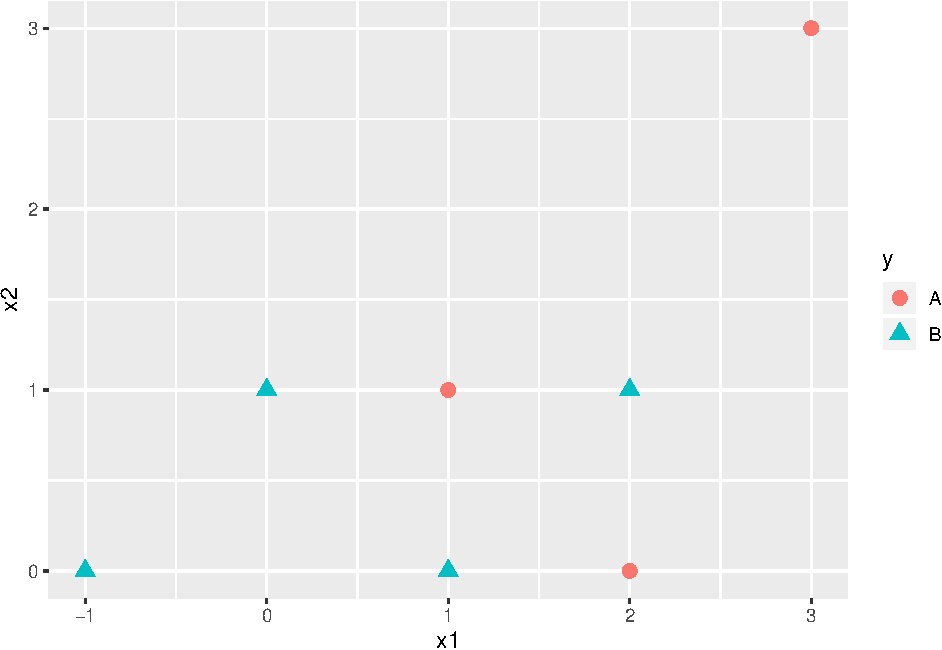
\includegraphics{2StatLearn.1_files/figure-beamer/unnamed-chunk-1-1.pdf}

\end{block}

\end{frame}

\begin{frame}

\begin{block}{Q: What are advantages and disadvantages of parametric and
non-parametric methods?}

\vspace{2mm}

Hints: interpretability, amount of data needed, complexity, assumptions
made, prediction accuracy, computational complexity, over/under-fit.

\end{block}

\end{frame}

\begin{frame}

\begin{block}{A: Parametric methods}

\begin{longtable}[]{@{}ll@{}}
\toprule
\begin{minipage}[b]{0.47\columnwidth}\raggedright\strut
Advantages\strut
\end{minipage} & \begin{minipage}[b]{0.47\columnwidth}\raggedright\strut
Disadvantages\strut
\end{minipage}\tabularnewline
\midrule
\endhead
\begin{minipage}[t]{0.47\columnwidth}\raggedright\strut
Simple to use and easy to understand\strut
\end{minipage} & \begin{minipage}[t]{0.47\columnwidth}\raggedright\strut
The function \(f\) is constrained to the specified
form.\vspace{2mm}\strut
\end{minipage}\tabularnewline
\begin{minipage}[t]{0.47\columnwidth}\raggedright\strut
Requires little training data\strut
\end{minipage} & \begin{minipage}[t]{0.47\columnwidth}\raggedright\strut
The assumed function form of \(f\) will in general not match the true
function, potentially giving a poor estimate.\vspace{2mm}\strut
\end{minipage}\tabularnewline
\begin{minipage}[t]{0.47\columnwidth}\raggedright\strut
Computationally cheap\strut
\end{minipage} & \begin{minipage}[t]{0.47\columnwidth}\raggedright\strut
Limited flexibility\strut
\end{minipage}\tabularnewline
\bottomrule
\end{longtable}

\end{block}

\end{frame}

\begin{frame}

\begin{block}{A: Non-parametric methods}

\begin{longtable}[]{@{}ll@{}}
\toprule
\begin{minipage}[b]{0.47\columnwidth}\raggedright\strut
Advantages\strut
\end{minipage} & \begin{minipage}[b]{0.47\columnwidth}\raggedright\strut
Disadvantages\strut
\end{minipage}\tabularnewline
\midrule
\endhead
\begin{minipage}[t]{0.47\columnwidth}\raggedright\strut
Flexible: a large number of functional forms can be fitted\strut
\end{minipage} & \begin{minipage}[t]{0.47\columnwidth}\raggedright\strut
Can overfit the data\vspace{2mm}\strut
\end{minipage}\tabularnewline
\begin{minipage}[t]{0.47\columnwidth}\raggedright\strut
No strong assumptions about the underlying function are made\strut
\end{minipage} & \begin{minipage}[t]{0.47\columnwidth}\raggedright\strut
Computationally more expensive as more parameters need to be
estimated\vspace{2mm}\strut
\end{minipage}\tabularnewline
\begin{minipage}[t]{0.47\columnwidth}\raggedright\strut
Can often give good predictions\strut
\end{minipage} & \begin{minipage}[t]{0.47\columnwidth}\raggedright\strut
Much data are required to estimate (the complex) \(f\).\strut
\end{minipage}\tabularnewline
\bottomrule
\end{longtable}

\end{block}

\end{frame}

\begin{frame}{Prediction accuracy vs.~interpretability}

(we are warming up to the bias--variance trade--off)

\textbf{Inflexible} methods:

\begin{itemize}
\tightlist
\item
  Linear regression (M3)
\item
  Linear discriminant analysis (M4)
\item
  Subset selection and lasso (M6)
\end{itemize}

\textbf{Flexible} methods:

\begin{itemize}
\tightlist
\item
  KNN classification (M4), KNN regression, Smoothing splines (M7)
\item
  Bagging and boosting (M8), support vector machines (M9)
\item
  Neural networks (M11)
\end{itemize}

\end{frame}

\begin{frame}

\begin{block}{Why would I ever prefer an inflexible method?}

\(~\)

Example: Prediction of icome from ``Years of Education'' and
``Seniority''\vspace{2mm}

\centering
\includegraphics[width=0.45000\textwidth]{../../ISLR/Figures/Chapter2/2.4.png}
\includegraphics[width=0.45000\textwidth]{../../ISLR/Figures/Chapter2/2.6.png}

A linear model vs a perfect fit.

\end{block}

\end{frame}

\begin{frame}

The choice of a flexible or inflexible method depends on the goal in
mind.

\begin{itemize}
\tightlist
\item
  For \textbf{inference} an inflexible model is easier to interpret.
\item
  For \textbf{prediction} a flexible model is more powerful.
\end{itemize}

\textbf{Overfitting} occurs when the estimated function \(f\) is too
closely fit to the observed data points.

\textbf{Underfitting} occurs when the estimated function \(f\) is too
rigid to capture the underlying structure of the data.

We illustrate this by a toy example using polynomial regression.

\end{frame}

\begin{frame}

\begin{block}{Polynomial regression example (simulation)}

Consider a covariate \(x\) observed between \(x=-2, \ldots , 4\) and
\(n=61\) observations.

\begin{center}\includegraphics{2StatLearn.1_files/figure-beamer/data-1} \end{center}

\end{block}

\end{frame}

\begin{frame}

We impose a relationship between reponse \(Y\) and covariate \(x\):

\[ Y=x^2 + \varepsilon\] with error (noise) term
\(\varepsilon\sim N(0,\sigma^2)\) with \(\sigma=2\). It is a substitue
for all the unobserved variables that are not in our equation, but that
might influence \(Y\).

We call \(Y=x^2\) the \emph{truth}.

\end{frame}

\begin{frame}

\begin{center}\includegraphics{2StatLearn.1_files/figure-beamer/truth-1} \end{center}

\end{frame}

\begin{frame}

Next, we want to fit a function to the observations \emph{without}
knowing the true relationship, and we have tried different parametric
polynomial functions.

\begin{itemize}
\item
  \textbf{poly1}: Simple linear model of the form \(\beta_0+\beta_1 x\)
  fitted to the observations. \emph{Underfits} the data.
\item
  \textbf{poly2}: Quadratic polynomial fit to the data, of the form
  \(\beta_0+\beta_1 x +\beta_2 x^2\). This fits well.
\item
  \textbf{poly10}: Polynomial of degree 10 fit of the form
  \(\beta_0+\beta_1 x +\beta_2 x^2+\cdots +\beta_{10}x^{10}\)
  \emph{Overfits} the data.
\item
  \textbf{poly20}: Polynomial of degree 10 fit of the form
  \(\beta_0+\beta_1 x +\beta_2 x^2+\cdots +\beta_{20}x^{20}\)
  \emph{Overfits} the data.
\end{itemize}

We will discuss polynomial regression in M7.

\end{frame}

\begin{frame}

\begin{center}\includegraphics{2StatLearn.1_files/figure-beamer/overunderfit-1} \end{center}

The degree of the polynomial is a \emph{flexibility parameter}.

\end{frame}

\begin{frame}

We can now ask:

\begin{itemize}
\item
  Which of these models performs ``best''?
\item
  Is there \emph{one} method that dominates all others?
\end{itemize}

\end{frame}

\begin{frame}{Assessing model accuracy}

\textbf{No method} dominates all others over all possible data sets.

\begin{itemize}
\tightlist
\item
  That is why we need to learn about many different methods.
\item
  For a given data set we need to know how to decide which method
  produces the \emph{best} results.
\item
  We need to understand what \emph{best} means.
\item
  How close is the predicted response to the true response value?
\end{itemize}

\end{frame}

\begin{frame}

\begin{block}{Measuring the Quality of Fit}

\begin{itemize}
\item
  A popular measure for the quality of fit: \emph{Training MSE} (mean
  squared error).
\item
  It is the mean of squared differences between prediction and truth for
  the training data (the same values that were used to estimate \(f\)):
\end{itemize}

\[ \text{MSE}_{\text{train}}=\frac{1}{n}\sum_{i=1}^n (y_i-\hat{f}(x_i))^2\]

\begin{itemize}
\tightlist
\item
  But: we are \emph{not} interested in how the method works on the
  training data. We want to know how good the method is when we use it
  on \emph{previously unseen test data} (e.g., future data).
\end{itemize}

\end{block}

\end{frame}

\begin{frame}

Examples:

\begin{itemize}
\item
  We don't want to predict last weeks stock price, we want to predict
  the stock price next week.
\item
  We don't want to predict if a patient in the training data has
  diabetes (because we already know this), we want to predict if a new
  patient has diabetes.
\end{itemize}

\end{frame}

\begin{frame}

\begin{center}\includegraphics[width=0.8\linewidth]{2StatLearn.1_files/figure-beamer/trainMSE-1} \end{center}

\textbf{Q}: Based on the training MSE - which model fits the data the
best?

Polynomial example: fitted order 1-20 polynomial when the truth is order
2. Left: one repetition, right: 100 repetitions of the training set.

\end{frame}

\begin{frame}

\begin{block}{Test MSE}

\begin{itemize}
\item
  Simple solution: estimate \(\hat{f}\) using the training data (maybe
  my minimizing the training MSE), but choose the \emph{best} model
  using a separate \emph{test set}.
\item
  \emph{Test MSE} for a set of \(n_0\) test observations
  \((x_{0j},y_{0j})\):
\end{itemize}

\[ \text{MSE}_{\text{test}}=\frac{1}{n_0}\sum_{j=1}^{n_0} (y_{0j}-\hat{f}(x_{0j}))^2\]

\begin{itemize}
\tightlist
\item
  Alternative notation: \[\text{Ave}(y_0-\hat{f}(x_0))^2\] (taking the
  average over all available test observations).
\end{itemize}

\end{block}

\end{frame}

\begin{frame}

\textbf{Q:} What if we do not have access to test data?

\vspace{2mm}

\textbf{Q:} But, can we instead just use the training data MSE to choose
a model? A low training error should also give a low test error?

\end{frame}

\begin{frame}

\begin{center}\includegraphics[width=0.9\linewidth]{2StatLearn.1_files/figure-beamer/traintestMSE-1} \end{center}

Polynomial example: fitted order 1-20 when the truth is order 2. Left:
one repetition, right: 100 repetitions for the testMSE.

\textbf{Q}: Based on the test MSE - which model fits the data the best?

\end{frame}

\begin{frame}

\begin{center}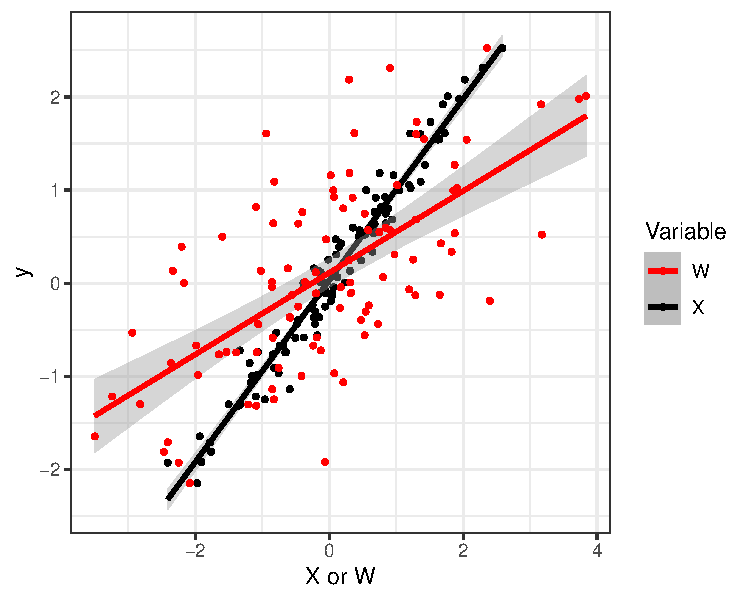
\includegraphics{2StatLearn.1_files/figure-beamer/unnamed-chunk-2-1} \end{center}

\textbf{A}: If choosing flexibility based on training MSE=poly20 wins,
if choose flexibility based on test MSE=poly 2 wins.

\end{frame}

\begin{frame}

\begin{block}{Test error vs.~training error}

\(~\)

Important observations:

\begin{itemize}
\item
  The test error seems to have a minimum (U-shape) in between the
  extremes.
\item
  The training error keeps going down.
\end{itemize}

\vspace{1.5cm} \centering
Why?

\end{block}

\end{frame}

\begin{frame}{The Bias-Variance trade-off}

\begin{itemize}
\item
  The U-shape is the result of \emph{two competing properties} of
  statistical learning methods.
\item
  Assume we have fitted a \emph{regression} curve
  \[Y  = f(x) + \varepsilon\] to our training data \(\{x_i, y_i\}\) for
  \(i=1,..,n\), and \(\varepsilon\) is an unobserved random variable
  that adds random, uncorrelated noise with mean zero and constant
  variance \(\sigma^2\). \(\varepsilon\) is a substitute for all the
  unobserved variables that influence \(Y\).
\item
  The training data was used to estimate \(\hat{f}\).
\end{itemize}

\end{frame}

\begin{frame}

\begin{itemize}
\item
  We want to use \(\hat{f}\) to obtain the predicted response value
  \(\hat{f}(x_0)\) for an unseed test observation \((x_0,y_0)\).
\item
  The \emph{expected test mean squared error (MSE) at \(x_0\)} is
  defined as: \[\text{E}[y_0 - \hat{f}(x_0)]^2\]
\end{itemize}

\(~\)

\begin{itemize}
\tightlist
\item
  Compare this to the test MSE for the polynomical example
  (\(\text{MSE}_{\text{test}}\)): The average is simply replaced by the
  \emph{theoretical version} (expected value).
\end{itemize}

\end{frame}

\begin{frame}

Using that \(y_0=f(x_0)+\varepsilon\), this expected test MSE can be
decomposed into three terms

\begin{align*}
&\text{E}[y_0 - \hat{f}(x_0)]^2 = \\
& ... \\
& =  \underbrace{\text{Var}(\varepsilon)}_{\text{Irreducible error}} + \underbrace{\text{Var}(\hat{f}(x_0))}_{\text{Variance of prediction}} + \underbrace{\left( f(x_0) - \text{E}[\hat{f}(x_0)] \right)^2}_{\text{Squared bias}}
\end{align*}

\textbf{Q}: what assumptions have we made in the derivation above?

\textbf{A}: classnotes.

\end{frame}

\begin{frame}

\[\text{E}[(y_0 - \hat{f}(x_0))^2]=\cdots=\text{Var}(\varepsilon) +  \text{Var}(\hat{f}(x_0))+[\text{Bias}(\hat{f}(x_0))]^2\]

\begin{itemize}
\item
  \emph{\textcolor{red}{Irreducible error}}. This term cannot be reduced
  regardless how well our statistical model fits the data.
\item
  \emph{\textcolor{red}{Variance}} of the prediction at
  \(\hat{f}(x_0)\). Relates to the amount by which \(\hat{f}(x_0)\) is
  expected to change for different training data. If the variance is
  high, there is large uncertainty associated with the prediction.
\item
  \emph{\textcolor{red}{Squared bias}}. The bias gives an estimate of
  how much the prediction differs from the true mean. If the bias is low
  the model gives a prediction which is close to the true value.
\end{itemize}

\end{frame}

\begin{frame}

Note: \[\text{E}[(y_0 - \hat{f}(x_0))^2]\]

is the \textbf{expected test MSE}. We can think of this as the average
test MSE we would obtain if we repeatedly estimated \(f\) using many
training sets (as we did in our example), and then tested this estimate
at \(x_0\).

However, if we also assume that \(X\) is a random variable, this is
really \(\text{E}[(Y - \hat{f}(x_0))^2 \mid X=x_0]\)

The \textbf{overall expected test MSE} can we then compute by averaging
the expected test MSE over all possible values of \(x_0\) (averaging
with respect to frequency in test set), or mathematically by the law of
total expectation \(\text{E} \{ \text{E}[(Y - \hat{f}(X))^2 \mid X]\}\)
(also sometimes referred to as the law of double expectations).

\end{frame}

\begin{frame}

\begin{block}{General rule}

\vspace{4mm}

For more flexible models, the variance will \emph{increase} and the bias
will \emph{decrease}.

\vspace{4mm}

\centering
This is called the \emph{\textcolor{red}{Bias-variance trade-off}}.

\end{block}

\end{frame}

\begin{frame}

\begin{block}{Polynomial example (cont.)}

\(Y=x^2\) is still the \emph{truth}.

\begin{center}\includegraphics[width=0.9\linewidth]{2StatLearn.1_files/figure-beamer/biasvarianceforx-1} \end{center}

For four different polynomial models (poly1,2,10 and 20), the squared
bias, variance, irreducible error and the total sum. Plots based on 100
simulations for the polynomial example.

\end{block}

\end{frame}

\begin{frame}

\begin{center}\includegraphics{2StatLearn.1_files/figure-beamer/biasvarianceforpoly-1} \end{center}

At four different values for \(x_0\), the squared bias, variance,
irreducible error and the total sum. Plots based on 100 simulations for
the polynomial example.

\end{frame}

\begin{frame}

\begin{center}\includegraphics[width=0.9\linewidth]{2StatLearn.1_files/figure-beamer/averageoverxs-1} \end{center}

Overall version (averaging over 61 gridpoints of \(x\)).

\end{frame}

\begin{frame}

\begin{block}{Choosing the best model}

\(~\)

When fitting a statistical model the aim is often to obtain \textbf{the
most predictive model}.

\begin{itemize}
\item
  \textbf{Training set}: The observations used to fit the statistical
  model \(\rightarrow\) Training error
\item
  \textbf{Test sample}: new observations which were not used when
  fitting the model \(\rightarrow\) Test error
\item
  Training error decreases for more complex models, but the test error
  has an \textbf{optimum}.
\item
  This trade-off in selecting a model with the right amount of
  complexity/flexibility is the \textbf{Bias-Variance trade-off}.
\end{itemize}

\end{block}

\end{frame}

\begin{frame}

\includegraphics{../../ISLR/Figures/Chapter2/2.12.png}

\begin{itemize}
\tightlist
\item
  Inflexible models may lead to a poor fit (high bias)
\item
  Flexible (complex) models may provide more unbiased fits but may
  overfit the data (high variance)
\item
  The aim is to find the optimum.
\end{itemize}

\end{frame}

\begin{frame}{References}

\hypertarget{refs}{}
\hypertarget{ref-ISL}{}
James, Gareth, Daniela Witten, Trevor Hastie, and Robert Tibshirani.
2013. \emph{An Introduction to Statistical Learning}. Vol. 112.
Springer.

\end{frame}

\end{document}
